\chapter{Vorstellung und Anwendung der Kriterien}
\label{chapter:kriterien}

In Kapitel \ref{chapter:grundlagen} wurden für die weitere Betrachtung der Streaming Frameworks notwendige Grundbegriffe erläutert und ein Referenzmodell wie in Abbildung \ref{fig:basismodell} gezeigt vorgestellt. Zunächst wird der Markt anhand der Studie \citelit{studie:bidama} im Kontext von Big Data in dem Streaming Frameworks zum Einsatz kommt vorgestellt. Die Studie \citelit{studie:bidama} wurde von Markl et al. im Auftrag des Bundesministeriums für Wirtschaft und Energie (BMWi) 2013 erstellt. 

\begin{quote}
Zentrales Ziel der vorliegenden Studie ist eine qualitative und quantitative Bewertung des Ist-Zustandes sowie der wirtschaftlichen Potenziale von neuen Technologien für das Management von Big Data. Daraus werden standortspezifische Chancen und Herausforderungen für Deutschland abgeleitet. In der Studie werden insbesondere auch rechtliche Rahmenbedingungen anhand von Einzelfällen betrachtet. Die Studie beinhaltet zudem konkrete Handlungsempfehlungen. 
\citelit[S. 3]{studie:bidama}
\end{quote}

Big Data wurde im Artikel \citelit{laney:threevs} von Laney 2001 in drei Dimensionen \textit{volume}, \textit{velocity} und \textit{variety} eingeordnet. Die Dimension \textit{volume} beschreibt den Umgang mit dem rasanten Anstieg an Datentransaktionen. \textit{Velocity} gibt die Geschwindigkeit an und \textit{variety} gibt die steigende Vielfalt der Daten an. In der Abbildung \ref{fig:bigdatacube} werden die drei Dimensionen in einem Würfel dem \textit{Big Data Cube} dargestellt. Die Abbildung \ref{fig:bigdatacube} wurde aus \citelit[S. 1, Abb. 1]{meijer2012your} in einfacher Form übernommen. So beschreibt Meijer \textit{volume} von klein \textit{small} nach groß \textit{big}, \textit{velocity} von ziehen \textit{pull} nach drücken \textit{push} und \textit{variety} von komplexen strukturierten Daten Fremd-/Primärschlüssel \textit{\acrshort{glo:fk}/\acrshort{glo:pk}} nach einfachen Zeigern auf Daten und Daten \textit{\acrshort{glo:k}/\acrshort{glo:v}}. Das herkömmliche relationale Datenbanksystem ist in der Abbildung \ref{fig:bigdatacube} unter den Koordinaten (\textit{small}, \textit{pull}, \textit{fk/pk}) zu finden. Unter den Koordinaten (\textit{small}, \textit{pull}, \textit{k/v}) wären Anwendungen zu finden, die das Konzept \textit{\gls{glo:orm}} implementieren. Beim Konzept \textit{\gls{glo:orm}} werden Objekte in relationalen Datenbanken abgebildet \citelit[S. 1]{meijer2012your}. Die Streaming Frameworks werden unter den Koordinaten (\textit{big}, \textit{push}, \textit{fk/pk}) eingeordnet. Gegenüber den Streaming Frameworks unter den Koordinaten (\textit{big}, \textit{pull}, \textit{fk/pk}) befinden sich die Batch Processing Engines, wie zum Beispiel Apache Hadoop \citeint{hadoop:home}. In der unteren linken Ecke (big, pull, k/v) werden Lambda Ausdrücke eingeordnet. Lambda Ausdrücken werden anonyme Methoden möglich. Damit können einfache Abfragen auf Sammlungen formalisiert werden. Der Compiler erzeugt zur Laufzeit die Methoden im Hintergrund. In Java stehen die Lambda Ausdrücke erst ab Version 8 zur Verfügung \citeint{res:oracle:java8}.

\begin{figure}[htb!]
\centering
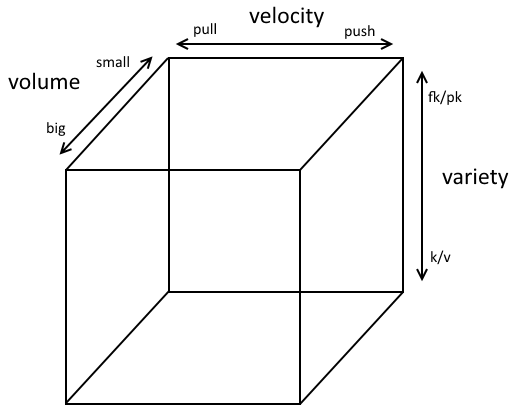
\includegraphics[width=1.0\textwidth]{bilder/bigdatacube.png}
\caption{Darstellung Big Data Cube
\label{fig:bigdatacube}}
\end{figure}

Relationale Datenbanksysteme stoßen im Zusammenhang der horizontalen Skalierung in der zentralisierten Systemarchitektur auf Probleme, wenn die Datenmenge die Kapazität einer Maschine übersteigt und dadurch das Ergebnis in keiner akzeptablen Zeit zurückgegeben wird \citelit[S. 30, Kap. 2.2.1]{edlich:nosql}. So zeigt Edlich et al. in dem Buch \citelit{edlich:nosql} einen alternativen Ansatz Daten zu halten. Dabei wird der Begriff \textit{NoSQL} als nicht relationales Datenbanksystem eingeführt und definiert \citelit[S. 2, K 1.2]{edlich:nosql}. In Verbindung mit horizontaler Skalierung, Replikation und niedriger Reaktionszeit wird in \citelit[S. 30, K. 2.2]{edlich:nosql} das \gls{glo:cap}-Theorem erklärt. Beim CAP-Theorem besteht der Konflikt in der Konsistenz \textit{C}. Es gilt zu Entscheiden ob die Konsistenz gelockert wird oder nicht. Bei einer lockeren Konsistenz und damit einer hohen Verfügbarkeit und Ausfalltoleranz können in einem Verbindungsausfall alte Zustände zurückgegeben werden. Falls nicht gelockert wird kann der Umstand in Kraft treten, sehr lange Reaktionszeiten zu erhalten. %Out-of-order, Dropped, Duplicate Messages
Daher wurde das Konsistenzmodell \gls{glo:base} eingeführt. Es basiert auf einem optimistischen Ansatz. Eine Transaktion nimmt den Status konsistent nicht unmittelbar ein. Erst nach einer gewissen Zeitspanne ist die Transaktion konsistent. Dieses Verhalten wird als \textit{Eventually Consistancy} bezeichnet. Als Beispiel gibt Edlich et al. in \citelit[S. 33, K. 2.2.3]{edlich:nosql} replizierende Knoten in einer Systemarchitektur an. 
% 3V Darstellung, nächere Darstellung ACID(::CAP)->BASE %% --> CRDTs

So wurden in der Studie \citelit{studie:bidama} neben der Einführung in Big Data, Stärken, Schwächen, Chancen und Risiken für die Branchen Handel, Banken, Energie, Dienstleistungen, Öffentlicher Sektor, Industrie, Gesundheitssektor, Marktforschung, Mobilitätsleistungen, Energie und Versicherungen als tabellarische Übersicht in \citelit[S. 105, Tab. 18]{studie:bidama} ausgegeben. In \citelit[S. 107, Abb. 54]{studie:bidama} werden Branchenschwerpunkte abgeleitet. Die genannte Abbildung wird im folgenden Zitat textuell erneut wiedergegeben:

\begin{quote}
	\begin{enumerate}
		\item Entwicklung neuartiger Technologien, um eine skalierbare Verarbeitung von komplexen Datenanalyseverfahren auf riesigen, heterogenen Datenmengen mit hoher Datenrate zu realisieren
		\item Senkung der Zeit und Kosten der Datenanalyse durch automatische Parallelisierung und Optimierung von deklarativen Datenanalysespezifikationen
		\item Schaffung von Technologieimpulsen, die zur erfolgreichen weltweiten Kommerzialisierung von in Deutschland entwickelten, skalierbaren Datenanalysesystemen führen
		\item Ausbildung von Multiplikatoren im Bereich der Datenanalyse und der skalierbaren Datenverarbeitung, welche die Möglichkeiten von Big Data in Wissenschaft und Wirtschaft tragen werden
		\item Technologietransfer an Pilotanwendungen in Wissenschaft und Wirtschaft
		\item Schaffung eines Innovationsklimas durch Konzentration von kritischem Big Data Know-how, damit deutsche Unternehmen und Wissenschaft nicht im Schatten des Silicon Valleys stehen
		\item Interaktive, iterative Informationsanalyse für Text und Weiterentwicklung geeigneter Geschäftsmodelle zur Schaffung von Marktplätzen für Daten, Datenqualität und Verwertung von Daten
		\item Datenschutz und Datensicherheit
	\end{enumerate}
	\citelit[S. 107, Abb. 54]{studie:bidama}
\end{quote}

Aus den abgeleiteten Schwerpunkten können mehrere Kriterien für die Betrachtung der Streaming Frameworks in Kapitel \ref{chapter:vorstellung} und des Referenzmodells in Kapitel \ref{section:technologie} herangezogen werden. Zunächst werden die gewonnen Kriterien in einer Liste aufgezählt. Anschließend werden die einzelnen Kriterien als Bewertungskriterien für die weitere Untersuchung der Streaming Frameworks definiert. Daraufhin werden die Bewertungskriterien auf das Referenzmodell angewendet.

\begin{itemlist}{Bewertungskriterien}{liste:bewkrit}
	\item Architektur
	\item Prozesse und Threads
	\item Kommunikation
	\item Namenssystem
	\item Synchronisierung
	\item Pipelining und Materialisierung
	\item Konsistenz und Replikation	
	\item Fehlertoleranz
	\item Sicherheit	
	\item Erweiterung
	\item Qualität
\end{itemlist}

Die ermittelten Bewertungskriterien aus Liste \ref{liste:bewkrit} unterstützen die Feststellung eines Streaming Frameworks und des Referenzmodells. Damit die einzelnen Bewertungskriterien bei der Anwendung eindeutig und klar sind, werden diese zunächst definiert und zusätzlich erläutert.

\begin{description}
	\item[Architektur] stellt den verwendeten Architekturstil vor und ordnet in eine Systemarchitektur ein.
	\item[Prozesse und Threads] zeigen die Anwendung von blockierendem oder nicht blockierendem Zugriff, also einer Verbindung zwischen Client und einem Server. Während der Betrachtung wird der Einsatz der verteilten Verarbeitung in der eingesetzten Architektur geprüft.
	\item[Kommunikation] gibt die Form des Nachrichtenaustauschs zwischen Client und Servern an. Zum Austausch der Nachrichten kommen Nachrichtenprotokolle zum Einsatz. Dabei wird auf die Protokollschicht \textit{Middleware}-Protokoll eingegangen. Im \acrshort{glo:osi}-Modell entspricht die Sitzungs- und Darstellungsschicht einer \textit{Middleware}-Schicht \citelit[S. 148, Abb. 4.3 angepasstes Referenzmodell]{tanenbaum:vs}. Dabei werden unterschiedliche Strategien \gls{glo:rpc}, Warteschlangensysteme, Kontinuierliche Systeme und Multicast Systeme, die beim Nachrichtenaustauschs eingesetzt werden, innerhalb der \textit{Middleware}-Protokolle eingeordnet. Außerdem wird das Verbindungsmodell, die Nachrichtenstruktur und der Einsatz einer Protokollversionierung vorgestellt. Weiterhin wird die Unterstützung von unterschiedlichen Nachrichtenkodierungen und Statusverwaltung betrachtet.
	\item[Namenssystem] zeichnet den Ansatz eines Benennungssystems. Hierbei wird linear-, hierarchisch- oder attributbasiert klassifiziert.
	\item[Synchronisierung] beschreibt die verwendeten Algorithmenarten. 
	\item[Pipelining und Materialisierung] gibt eine Technik an, ob komplexe Aggregate berechnet werden und innerhalb der Abfragen wieder benutzt werden können.
	\item[Konsistenz und Replikation] zeigt die Skalierungstechnik auf und stellt die Verwaltung der Replikation vor. 	
	\item[Fehlertoleranz] zeigt das verwendete Fehlermodell und stellt eine Strategie im Wiederherstellungsfall vor.
	\item[Sicherheit] stellt das Konzept vor und beschreibt den Einsatz von sicheren Kanälen und der Zugriffssteuerung.	
	\item[Erweiterung] beschreibt Methoden weitere Systemarchitekturen anzuschließen.
	\item[Qualität] zeigt das verwendete Modell für die Dienstgüte.
\end{description}

In der Liste \ref{liste:bewkrit} wurden Bewertungskriterien vorgestellt und definiert, die nun auf das Referenzmodell aus Kapitel \ref{section:technologie} angewendet werden. In der Tabelle \ref{tab:bewrefaurbor} wird eine Übersicht über die Bewertung zum Referenzmodell Aurora Borealis gegeben. Als Architektur wird strukturierte Peer-to-Peer-Architektur angegeben. In einer dezentralisierten Architektur, wie es die strukturierte Peer-to-Peer-Architektur ist, werden Nachrichten zwischen den Rechnerknoten die auch Peers genannt werden, mit Hilfe von verteilten Hashtabellen ausgetauscht. Dabei übernimmt bei Aurora Borealis ein Knoten den Master bei dem Nachrichten von den Verarbeitungsknoten zurückkommen. So wird in Abbildung \ref{fig:aurborinaction} eine Anwendung gezeigt in der ein Server 1 die Datenverarbeitung auf zwei Datenverarbeitungsservern 2 und 3 ausführen lässt und das Ergebnis aus der Daten- und Verarbeitungsebene an einen Rechner 4 mit der Benutzerschnittstelle zurückschickt. \citelit[S. 64, Kap. 2.2.2]{tanenbaum:vs} 

Aus der strukturierten Architektur folgt die Frage wie Prozesse untereinander kommunizieren. Die Prozesse kommunizieren entweder lokal oder entfernt asynchron über \gls{glo:rpc}. Anfragen von entfernten Prozessen werden automatisch lokal übersetzt. Ein Rechnerknoten stellt damit eine vollständige Verarbeitungseinheit dar. Der Prozess muss also gleichzeitig als Client und als Server arbeiten und ist dadurch symmetrisch. \citelit[S. 6, Kap. 2]{borealis:developer}

\begin{table}[htbp]
	\centering
		\begin{tabular}{@{}ll@{}} \toprule
			\textbf{Kriterium} & \textbf{Bewertung} \\ \midrule
			Architektur & Strukturierte Peer-to-Peer-Architektur \\
			Prozesse und Threads & Interaktion symmetrisch \\ 
			Kommunikation &  Transportunabhängiges \gls{glo:rpc}\\
			Namenssystem &  Attributbasierte Benennung\\
			Synchronisierung &  Zentralisierter Algorithmus \\
			Pipelining und Materialisierung &  In/Out Attribut\\
			Konsistenz und Replikation & Push-basiertes Monitoring \\			
			Fehlertoleranz &  Replikation \\
			Sicherheit & Nur Verfügbarkeitsprüfung \\			
			Erweiterung & Nur Eigenentwicklung \\
			Qualität &  Monitor, Optimierer, Voruasberechnen, Lokal und Global\\
			\bottomrule			
		\end{tabular}
	\caption{Bewertung Referenzmodell Aurora Borealis}
	\label{tab:bewrefaurbor}
\end{table}

In der Kommunikation wird ein transportunabhängiges \gls{glo:rpc} angegeben \citelit[S. 7, Abb. 2.1]{borealis:developer}. So findet der Nachrichtenaustausch zwischen zwei entfernten Rechnern asynchron statt. Die entfernten Rechner entsprechen den Verarbeitungseinheiten. Zwischen einem führenden Rechner und einem entfernten Rechner werden zwei Nachrichten verschickt. Die erste Nachricht führt eine Aktion auf dem entfernten Rechner aus und die zweite Nachricht ist das Ergebnis das vom entfernten Rechner dem führenden Rechner zurück gegeben wird. Hierbei beschreibt Tanenbaum et al. in \citelit[S. 158, Kap. 4.2.3]{tanenbaum:vs} den Nachrichtenaustausch als verzögerter synchroner \gls{glo:rpc}. Das kontinuierliche Verarbeiten von Abfragen wird dabei von einem führenden Rechner der \textit{Middleware}-Schicht übernommen. Dem führenden Rechner dem \textit{Global Load Manager} \citelit[S. 28, Kap. 5]{borealis:developer} wird beim Start des Systems eine \textit{Topology} übergeben. Die \textit{Topology} enthält einen Ausführungsplan mit komplexen Abfragen. Der \textit{Global Load Manager} verwaltet die Auslastung der entfernten Rechner und gleicht hohe Last durch Umverteilung der Aufgaben auf andere Rechner aus. Jeder Verarbeitungseinheit besteht aus einem \textit{Availabilty Monitor} \citelit[S. 38, Abb. 7.2]{borealis:developer} dem Verfügbarkeitsmonitor, einem \textit{Load Manager} der mit dem \textit{Global Load Manager} kommuniziert und einem \textit{QueryProcessor} der die Abfrage ausführt \citelit[S. 10, Kap 3.2]{borealis:developer}. 

Bei der Anwendung einer Verarbeitung in Aurora Borealis wird eine Konfiguration in einer \gls{glo:xml}-Datei für die Verteilung der Abfragen benötigt. Im Quelltext \ref{lst:aurorborealisdeoployconf} wird eine Konfiguration für Zwei Verarbeitungseinheiten formuliert. Einer Verarbeitungseinheit wird die Abfrage \textit{mycount} und der anderen Verarbeitungseinheit die Abfrage \textit{myfilter} zugeordnet. Beide Verarbeitungseinheiten abonnieren den Eingangsstrom \textit{stream} \textit{Aggregate} und veröffentlichen den \textit{stream} \textit{Packet} an die angegebene Verteilungseinheit. Für die Abfrage wird eine zustäzlich \gls{glo:xml}-Datei verwendet. In der Konfiguration \ref{lst:aurorborealisqueryconf} werden die Abfragen \textit{mycount} und \textit{myfilter} für die Zwei Verarbeitungseinheiten definiert. Die Abfrage wird im XML-Tag \textit{borealis} ausgezeichnet. Mit dem XML-Tag \textit{schema} werden komplexe Aurora Borealis Datentypen definiert. 

Die Benennung wird durch Attribute gekennzeichnet. Zum Beispiel hat das Schema \textit{PacketTuple} ein Feld mit dem Namen \textit{time} und den primitiven Datentypen \textit{int} in \gls{glo:coo}. Es werden Sechs Feldtypen (\textit{int}, \textit{long}, \textit{single}, \textit{double}, \textit{string}, \textit{timestamp}) unterstützt \citelit[S. 17, Tab. 4.2]{borealis:programmer}. Borealis erzeugt durch die \textit{Marshalling}-Anwendung eine \gls{glo:coo}-Struktur \textit{struct} vom Typ \textit{TupleHeader} \citelit[S. 37, Kap. 5.2.1]{borealis:programmer}. Die \textit{Marshalling}-Anwendung kapselt die komplexe auf \textit{Borealis} spezialisierte \gls{glo:nmstl} für \gls{glo:coo} \citelit[S. 35, Kap. 5.2]{borealis:programmer}. Der Quelltext \ref{lst:aurorborealismytest} zeigt die Methoden der \textit{Marshalling}-Anwendung für die beschriebenen Konfigurationen \ref{lst:aurorborealisdeoployconf} und \ref{lst:aurorborealisqueryconf}. In der Abfrage der ersten Verarbeitungseinheit wird im \gls{glo:xml}-Tag \textit{parameter} mit die Aggregatsfunktion \textit{count()} die Anzahl der Pakete jede Sekunde nach Zeit sortiert. Die Tabelle in \citelit[S. 23, Tab. 4.5]{borealis:programmer} zeigt eine Übersicht über die möglichen Aggregat-Parameter. Die zweite Abfrage filtert den Ausgabestrom aus der ersten Abfrage nach geraden Zeitwerten und gibt den Ausgabestrom \textit{Aggregate} zurück. Die Abbildung \ref{fig:aurborinaction} zeigt die Ausführung der Kommunikation.

\begin{figure}[htb!]
\centering
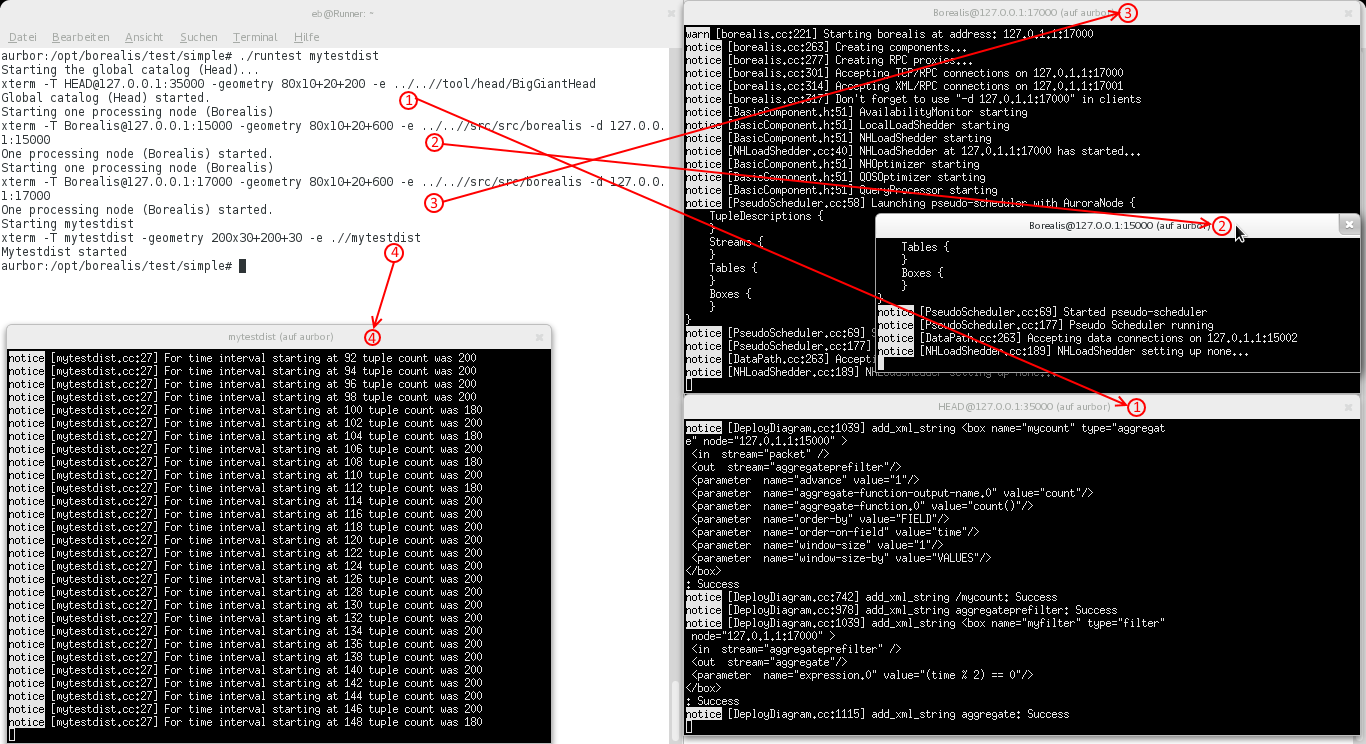
\includegraphics[width=1.0\textwidth]{bilder/auroraborealisinaction.png}
\caption{Aurora Borealis mit einem Master zwei Servern und einem Konsumenten
\label{fig:aurborinaction}}
\end{figure}

Pipelining wird durch den Einsatz von Eingangs- und Ausgangsstrom in Abfragen erreicht. In der Konfiguration \ref{lst:aurorborealisqueryconf} wird von der ersten Einheit ein spezialisiertes Datentupel \textit{AggregatePreFilter} erzeugt und die zweite Einheit bezieht das Ergebnis und verändert es. Zusätzlich können über eine \textit{Map}-Funktion in der Abfrage mehrere Datenströme erzeugt und komplex verarbeitet werden \citelit[S. 20, Kap. 4.9.1]{borealis:programmer}.

Die Konsistenz in den Verarbeitungseinheiten wird mit dem \textit{Consistancy Manager} erreicht. Durch die zusätzliche Komponente \textit{Availability Monitor} werden Statusinformation zwischen den Einheiten ausgetauscht. Einzelne Verarbeitungseinheiten können repliziert werden. Die Konfiguration der Replikation wird in der Konfiguration \ref{lst:aurorborealisdeoployconf} hinzugefügt. Im Gegensatz zum \gls{glo:xml}-Tag \textit{box} wird bei der Replikation \textit{replica\_set} verwendet. Die Abfrage wird ebenfalls dem \textit{replica\_set} zugeordnet. Innerhalb des \textit{replica\_set} werden einzelne \textit{node}-Elemente mit Zieladresse hinterlegt. Durch die Replikation wird in Aurora Borealis Fehlertoleranz erreicht. \citelit[S. 34, Kap. 7]{borealis:developer}

In der Sicherheit werden keine Sicherheitsrichtlinien vorgestellt und angewendet. Die Kommunikation zwischen einzelnen Rechnern findet unverschlüsselt auf TCP-Ebene über RPC statt. Eine Authentifizierung und Autorisierung wird nicht durchgeführt. Eine leichtgewichtichtete Kontrolle kann durch den \textit{Consistancy Manager} und dem \textit{Availability Monitoring} als Protokollwerkzeuge angesehen werden. Für komplexe Kontrollen ist eine eigene Implementierung notwendig \citelit[S. 38, Kap. 7.2.2]{borealis:developer}.

Erweiterungen können durch eigene Entwicklung in den bestehende Quelltext hinzugefügt werden. Methoden für weitreichende Abfragen in andere Umgebungen wie zum Beispiel Python sind nicht vorhanden. Eine umfangreiche Testabdeckung und eine gute Dokumentation für bestehende Methoden sind vorhanden. Das Erstellen von Aurora Borealis wurde bisher nur auf einer älteren Linux-Distribution durchgeführt. Der Quelltext in der letzten Version 2008 ist auf den Linux Compiler Version 3.1.1 angepasst und muss beim Einsatz der aktuellen Compiler-Version aktualisiert werden. Im Anhang \ref{sec:aurborinstall} wird eine ausführliche Anleitung zur Installation von Aurora Borealis in der aktuellen Version 2008 mit einer älteren Debian-Distribution vorgestellt. Der Quelltext von Aurora Borealis und die verwendete Debian-Version liegt im Verzeichnis \textit{anhangSoftwareZusatz} bei. Eine lauffähige virtuelle Maschine steht ebenfalls im gleichen Verzeichnis bereit.

Die Qualität der Dienste wird in Aurora Borealis durch verschiedene Mechanismen erreicht. Lokal werden pro Rechnereinheit mit dem \textit{Local Monitor} Statuswerte von \gls{glo:cpu}, Festplatte, Bandbreite und Energieversorgung erfasst und an den globalen \textit{End-point Monitor }übertragen. Der \textit{End-point Monitor} wertet die Qualität des Dienstes aus und führt eine Statistik pro Erfassung. Optimiert wird lokal durch den \textit{Local Monitor} mit dem \textit{Local} und \textit{Neighborhood Optimizer} und global durch den \textit{Global Optimizer}. Probleme werden durch die Monitore erkannt. Da jedem Datentupel ein \textit{Vector of Metrics} dazugeschaltet ist und es möglich ist zusätzlich einen \textit{Vector of Weights} (Lifetime, Coverage, Throughput, Latency) dazuzuschalten, ist eine Berechnung der Ursache eines \gls{glo:qos}-Problems möglich. \citelit[S. 7, Kap. 5]{abadi2005design}

In diesem Kapitel wurden die Vier Vs in \textit{Big Data} vorgestellt und die Streaming Frameworks wurden darin in einem Vergleich zu relationalen Datenbanksystemen eingeordnet. Weiterhin wurden die Konsistenz und die Verfügbarkeit im Zusammenhang von CAP und BASE vorgestellt. Mit der Studie \citelit{studie:bidama} und \citelit{tanenbaum:vs} wurden Bewertungkriterien in der Liste \ref{liste:bewkrit} erarbeitet. Abschließend wurde ausgehend von den Bewertungskriterien das Referenzmodell Aurora Borealis ausgewertet. In Kapitel \ref{chapter:vorstellung} werden nun die Streaming Frameworks vorgestellt und mit Bewertungskriterien in Liste \ref{liste:bewkrit} ausgewertet.